\section{Développement de l'application mobile}
Notre mission est de réaliser une simple application sous Android qui utilise le système SIRAM pour reconnaître les matricules des véhicules au Maroc sur des images ou des vidéos en temps réel. Pour réaliser une application de qualité, il est important de passer par deux étapes primordiales: l'analyse des besoins et la conception.  
    \subsection{Analyse et spécification des besoins}
    Dans cette partie, nous allons tout simplement identifier les acteurs et leurs actions. Un acteur est une personne, une machine ou un autre système qui interagit avec le système étudié. Leurs différentes interactions avec le système constituent ce qu'on appelle cas d'utilisation.

    Pour ce qui concerne notre application, nous avons un unique acteur qui est l’\textbf{utilisateur}. Il peut accèder à l'application pour:
    \begin{itemize}
        \item \textbf{Capturer une image}: l’utilisateur peut lancer la caméra et prendre une capture d’une photo. Cette photo est ensuite automatiquement traitée par le système pour faire la reconnaissance des plaques d’immatriculation éventuellement détectées sur la photo. Le système renvoie sur l’écran de l’application le résultat en image.
        \item \textbf{Lancer le traitement en temps réel}: l’utilisateur peut encore lancer la caméra. Mais cette fois-ci, le système traite en temps réel les images reçues par la caméra. Il trace sur ces images les rectangles autour des plaques éventuelles sans oublier les numéros de matricule sur ces rectangles.
    \end{itemize}
    Pour représenter graphiquement ces fonctionnalités, nous allons utiliser ce qu’on appelle en langage UML le diagramme de cas d’utilisation. C’est un simple diagramme qui permet de décrire l’ensemble des opérations réalisables par un acteur. Ainsi notre diagramme de cas d’utilisation peut être représenté comme suit:
    \begin{figure}[H]
        \centering
        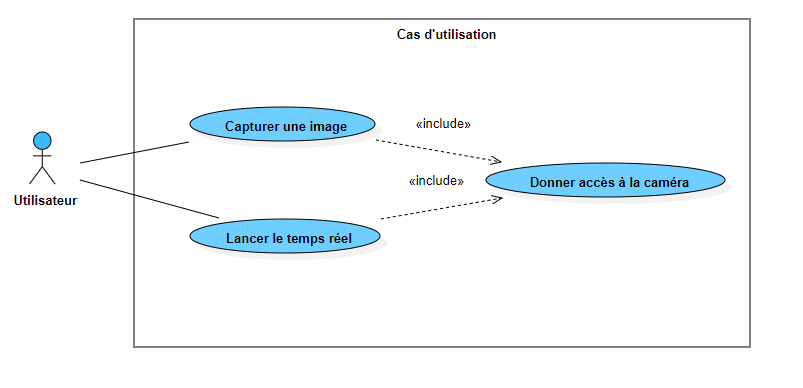
\includegraphics[scale=0.6]{useCase.png}
        \caption{Diagramme de cas d'utilisation}
    \end{figure}
    Ces fonctionnalités citées représentent les besoins fonctionnels de notre application. Hors mis ce type de besoins, nous avons aussi les besoins non-fonctionnelles qui sont un ensemble des contraintes à respecter par l'application. Dans notre cas, on a:
    \begin{itemize}
        \item \textbf{L'ergonomie des interfaces}: les interfaces de l'application doivent être simples et conviviales pour l'utilisateur. On doit aussi limiter au maximum les encombrements.
        \item \textbf{La performance}: il s'agit principalement de la précision et la rapidité de la reconnaissance des plaques. En effet, notre application doit détecter le plus rapidement possible les plaques et identifier le numéro de plaque avec une grande précision. 
    \end{itemize}

    \subsection{Conception}
    À partir d’une bonne analyse des besoins, on réalise la conception qui est l’une sinon la plus importante étape entrant dans le processus de développement d’une application. La conception se matérialise généralement par des diagrammes UML tels que les \textbf{diagrammes de classes}, les \textbf{diagrammes de séquence} et les \textbf{diagrammes d'activités}. Un diagramme de classes permet représenter les classes et les interfaces d'un systèmes ainsi que les relations entre elles. Contrairement à un diagramme de classes qui est statique, un diagramme de séquence est dynamique et traduit les intéractions entre acteurs et/ou le système pour un cas d'utilisation déterminé. Le déroulement d'un cas d'utilisation ou d'une méthode est présenté en utilisant un diagramme d'activités.
    
    
    Pour mieux structurer notre application et faciliter ainsi les modifications et les maintenances, nous avons opté pour une \textbf{architecture 3-tiers} (Figure \ref{fig:dc1}) c’est-à-dire composée de trois couches principales qui communiquent entre elles en offrant les services les unes aux autres:
    \begin{itemize}
        \item La \textbf{couche métier}: elle implémente la logique fonctionnelle de notre application. Elle est composée de plusieurs packages à savoir:
            \begin{itemize}
                \item[•] Le package \textbf{\textit{entities}}: qui contient les classes décrivant l'élément principal traité par notre application: la plaque d'immatriculation marocaine. Puisqu'il en existe plusieurs types, nous avons eu besoin de créer une classe abstraite qui prend en compte les caractéristiques et actions communes.
                
                \item[•] Le package \textbf{\textit{utils}}: qui contient des classes permettant de faire certains traitements sur les images ou des manipulations entrant dans le cadre du \textit{multithreading}.
                
                \item[•] Le package \textbf{\textit{detector}}: qui contient des classes permettant de localiser les plaques sur les images. Dans ce package, nous avons utilisé le \textbf{Design Pattern Builder} pour rendre plus flexible la création des détecteurs de plaques. Ceci pourra être utile si on veut par exemple utiliser une stratégie pour localiser les plaques autre que la détection des objets avec YOLO.
                
                \item[•] Le package \textbf{\textit{ocr}}: qui contient les classes servant à extraire les matricules sur les plaques localisées. Pour les besoins d'évolution et de modification ultérieure, nous avons fait appel à un couplage faible en utilisant les interfaces à la place des classes concrètes.
                
                \item[•] Le package \textbf{\textit{analysers}}: qui contient une classe regroupant le processus de détection et de lecture des plaques d'immatriculation. Ici on utilise le principe d'\textbf{injection de dépendances par constructeur} pour initialiser le détecteur de plaques et le lecteur OCR.
                
            \end{itemize}
        
        \item La \textbf{couche persistance}: elle gère l’accès aux données et principalement la communication avec la base de données. Elle a été implémentée à travers un package appelé \textbf{\textit{dao}}. Nous y avons utilisé le \textbf{Design Pattern Singleton} pour assurer la création d'une seule instance de l'objet communiquant avec la base de données. 
        
        \item La \textbf{couche présentation}: c’est la couche visible par l’utilisateur. Elle est composée des différentes interfaces graphiques de notre application. Nous les avons regroupées dans un seul package appelé \textbf{\textit{ui}}. Ce package contient deux classes. Une décrivant la page principale et une autre décrivant la page secondaire où se réalise la reconnaissance des plaques en temps réel. 
    \end{itemize}
    Cette architecture est illustrée à travers le diagramme de classes dans la figure \ref{fig:dc1}. La figure \ref{fig:ds1} montre comment l'utilisateur interagit avec le système à l'aide d'un diagramme de séquence. La figure \ref{fig:da1} est un diagramme d'activités représentant le déroulement de la reconnaissance des plaques en temps réel par le système.
    
    \subsection{Réalisation}
    Le développement de notre application mobile Android a été effectué en utilisant plusieurs outils matériels et logiciels. Sur le côté matériel, nous avons utilisé un PC dont les caractéristiques sont les suivantes:
        \begin{itemize}
            \item \textbf{Système d'exploitation 64 bits Windows 10};
            \item \textbf{Un disque dur SSD 237 Go};
            \item \textbf{Une mémoire RAM de 8 Go};
            \item \textbf{Un processeur Intel(R) Core(TM) i5-10210U CPU @ 1.60GHz   2.11 GHz}.
        \end{itemize}
    
    Les outils logiciels utilisés pour la réalisation de l’application sont:
    \begin{itemize}
        \item \textbf{Android Studio}: c’est un puissant environnement de développement (IDE) des applications Android créé par les ingénieurs de JetBrains et de Google. Tout le développement de notre application s’est fait sur cette plateforme. 
        
        \item \textbf{Kotlin/Java}: pour développer les applications Android, on peut utiliser soit le langage de programmation Java soit le langage Kotlin ou même les deux à la fois. Presque similaires, ces deux langages sont interopérables: on peut appeler les méthodes d'une classe Java dans une classe Kotlin et vis versa. En ce qui nous concerne, nous avons choisi le langage Kotlin comme notre langage principal de développement d’une part parce que c’est le langage officiel conseillé par Google pour le développement des applications sous Android. D’autre part, nous avons préféré Kotlin à Java pour la simplicité de sa syntaxe qui rend le code moins verbeux. Par ailleurs, l’ajout de certains extensions comme \textbf{les Data Class, les coroutines} qui facilitent énormément le développement. Néanmoins nous avons utilisé certaines classes utiles écrites en Java par d'autres développeurs.  
        
        \item \textbf{SQLite}: pour la base de données, nous avons opté pour SQLite qui un système de gestion de base de données à la fois puissant et léger et donc adapté pour une application mobile. Et comme recommandé par la documentation d'Android \cite{androiddocs}, nous avons utilisé la bibliothèque de persistence \textbf{\textit{Room}} qui fournit une couche d'abstraction sur SQLite pour permettre un accès fluide à la base de données.
        L'architecture de la bibliothèque \textit{Room} est décrite dans le figure \ref{fig:room}.

        \item \textbf{CameraX}: c'est une bibliothèque proposée par Android qui facilite l'utilisation de la Camera dans les applications Android. Elle offre déjà des services notamment \textbf{\textit{Image Analysis}} qui permet de faire des opérations de Machine Learning. Nous l'avons utilisé pour le cas de la reconnaissance en temps réel pour traiter chaque \textit{frame} renvoyé par la caméra.
        
        \item \textbf{Tensorflow Lite}: c'est un API développé par Google pour déployer facilement les modèles de Machine Learning sur les appareils mobiles. Nous l'avons donc utilisé pour déployer nos deux modèles YOLO. Mais au préalable, nous avons converti les modèles du format YOLO en format TFLite (format reconnu par l'API).
        
        \item \textbf{Git/GitHub}: pour conserver l’historique des modifications de notre code et collaborer avec les autres, nous avons opté pour le logiciel connu et apprécié Git. Pour héberger le code et conserver l’historique des modifications sur le Cloud, nous avons utilisé la plateforme GitHub. Nous y avons créé un répertoire privé qui contient les différentes versions du code de l’application.
    \end{itemize}
    \begin{figure}
        \centering
        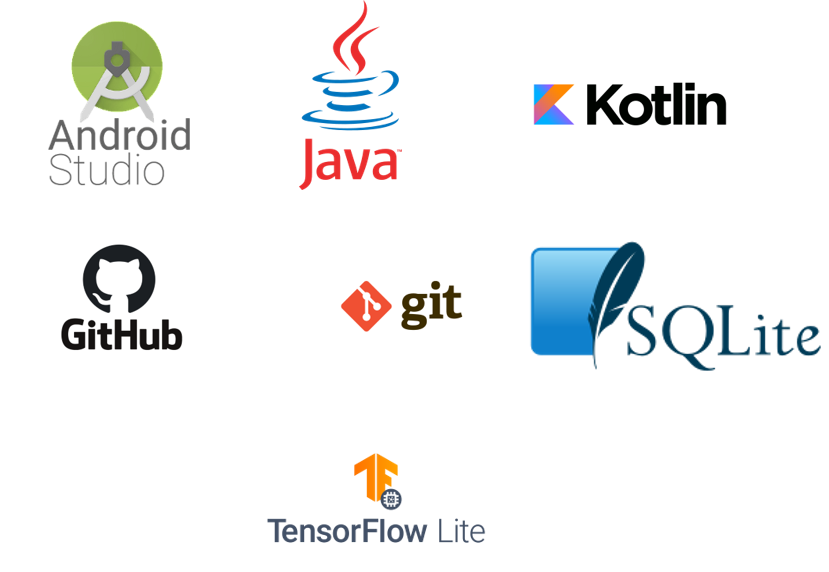
\includegraphics[scale=0.6]{logicielMobile.png}
        \caption{Quelques outils logiciels pour le développement de l'application mobile}
    \end{figure}
La combinaison de ces outils nous a permis de développer une application simple, performante et facile à prendre en main dont voici quelques interfaces:
\begin{figure}[H]
    \begin{subfigure}{0.3\textwidth}
        \centering
        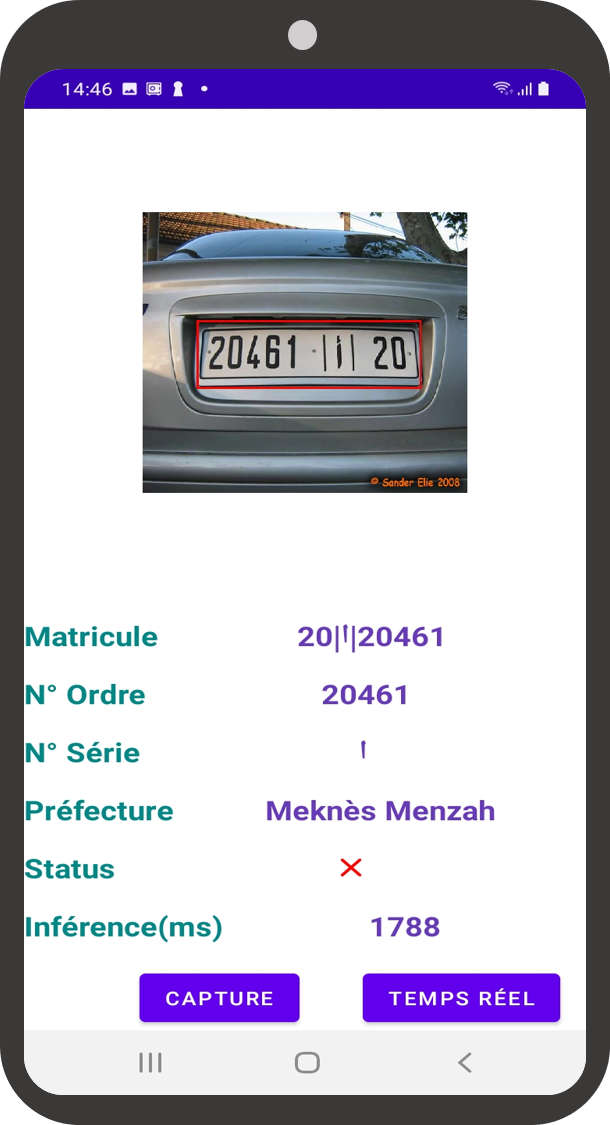
\includegraphics[width=\textwidth]{interface1.png}
        \caption{Exemple d'une reconnaissance de plaque non enregistrée dans la base de données réalisée en 1788 ms}
    \end{subfigure}
    \hfill
    \begin{subfigure}{0.3\textwidth}
        \centering
        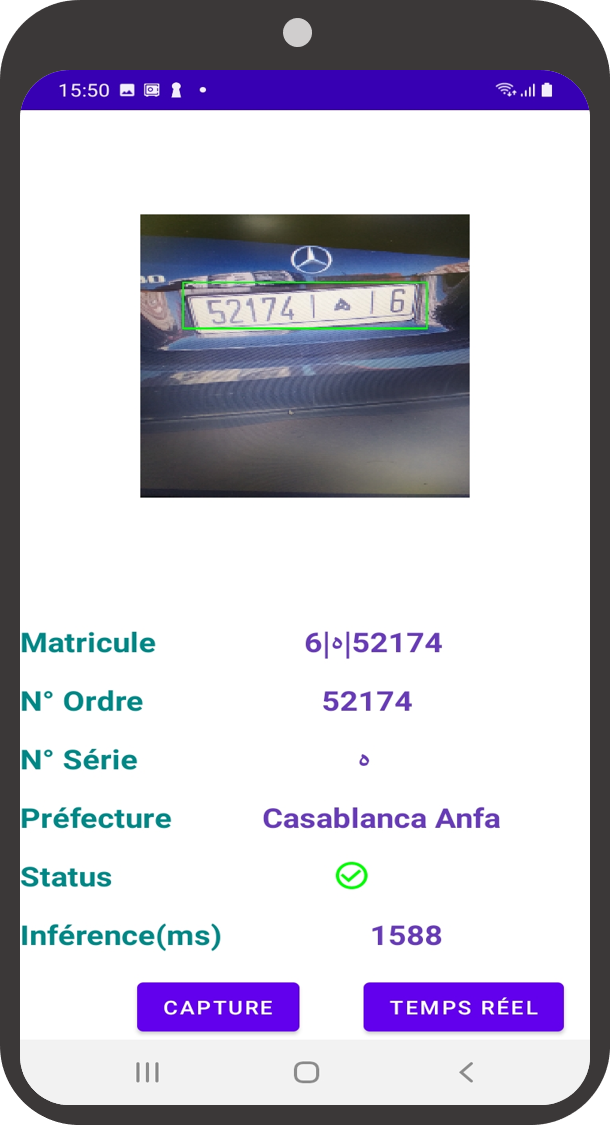
\includegraphics[width=\textwidth]{interface2.png}
        \caption{Exemple d'une reconnaissance de plaque enregistrée dans la base de données réalisée en 1588 ms}
    \end{subfigure}
    \caption{Exemples de quelques interfaces de l'application mobile}
\end{figure}


